\documentclass[11pt, letterpaper]{article}
\usepackage[utf8]{inputenc}
\usepackage[letterpaper, margin=0.5in]{geometry}
\usepackage{amsmath}
\usepackage{amssymb}
\usepackage{amsthm}
\usepackage{graphicx}
\usepackage{listings}
\usepackage[font=scriptsize]{caption}
\usepackage{subcaption}
\usepackage{xcolor}

\newtheorem{lemma}{Lemma}
\newcommand{\indep}{\perp \!\!\! \perp}

\definecolor{codegreen}{rgb}{0,0.6,0}
\definecolor{codegray}{rgb}{0.5,0.5,0.5}
\definecolor{codepurple}{rgb}{0.58,0,0.82}
\definecolor{backcolour}{rgb}{0.95,0.95,0.92}

\lstdefinestyle{mystyle}{
    backgroundcolor=\color{backcolour},   
    commentstyle=\color{codegreen},
    keywordstyle=\color{magenta},
    numberstyle=\tiny\color{codegray},
    stringstyle=\color{codepurple},
    basicstyle=\ttfamily\footnotesize,
    breakatwhitespace=false,
    texcl=true,
    mathescape=true,
    breaklines=true,                 
    captionpos=b,                    
    keepspaces=true,                 
    numbers=left,                    
    numbersep=5pt,                  
    showspaces=false,                
    showstringspaces=false,
    showtabs=false,                  
    tabsize=2
}

\lstset{style=mystyle}
\graphicspath{ {../statics/} }
\captionsetup{justification=raggedright, singlelinecheck=false}

\author{Ryan Tang}
\title{STA 532 HW 5}
\date{February 20th 2023}

\begin{document}
\maketitle

\section{Chapter 2 Ex 3}
Tropical cyclone study. Here we have the annual counts $X = (X_1 \dots X_n), X_j \thicksim_{iid} \text{Poisson}(\alpha\beta^{j-1})$
\paragraph{(a)} Sufficiency
\begin{align*}
    p(X|\theta=(\alpha, \beta)) &= \prod_j^n \text{Poisson}(X_j|\alpha \beta^{j-1}) \\
        &= \prod_j^n (X_j!)^{-1} (\alpha\beta^{j-1})^{X_j} \exp(-\alpha\beta^{j-1}) \\
        &= (\prod_j^n X_j!)^{-1} (\frac{\alpha}{\beta})^{\sum X_j} \beta^{\sum jX_j} \exp(-\alpha \sum \beta^{j-1})
\end{align*}
Hence, the sufficient statistics $T(X) = (\sum X_j, \sum jX_j)$ follows the factorization theorem.
\begin{align*}
    p(X|\theta=(\alpha, \beta))
        &= (\prod_j^n X_j!)^{-1} (\frac{\alpha}{\beta})^{\sum X_j} \beta^{\sum jX_j} \exp(-\alpha \sum \beta^{j-1}) \\
        &= h(X) c(\theta) (\frac{\alpha}{\beta})^{\sum X_j} \beta^{\sum jX_j} \\
        &= h(X) c(\theta) (\frac{\alpha}{\beta})^{t_1} \beta^{t_2} \\
        &= h(X) g(T(X), \theta)
\end{align*}

\paragraph{(b)}
Using the sufficient statistics, we plot the log-likelihood $g(T(X), \theta)$ in Figure \ref{fig:sufficient-logl} and constrained under the region that we have at least 15\% of the maximum log-likelihood score from $(\hat{\alpha}, \hat{\beta}) = (7.06, 1.0042)$. The square region is simply an estimation through discrete approximation. The range of $\alpha$ is $(0.4, 67.65)$ and the range of $\beta$ is $(0.95, 1.05)$.
\begin{figure*}[!h]
  \centering
  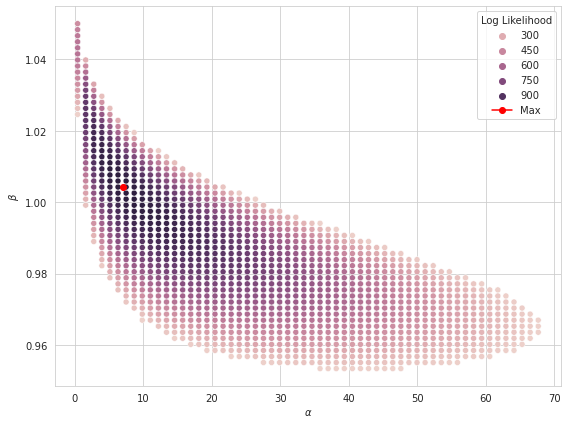
\includegraphics[width=0.6\textwidth]{hw5-1.png}
  \captionsetup{justification=centering}
  \caption{The discrete estimation of the un-normalized log-likelihood function $g(T(x), \theta)$ using the sufficient statistics. We only plotted the points in that we have at least 15\% of the maximum log-likelihood score to highlight the region.}
  \label{fig:sufficient-logl}
\end{figure*}

\paragraph{(c)}
I think if we carry out a traditional hypothesis test with a null hypothesis $H_0: \beta = 1$ and fail to reject the null based on the 100 observations still doesn't answer the question of whether there is a positive or negative trend. It only says we don't have enough evidence to make a claim. In my opinion, and a more intuitive way of answering the question, it is more sensible to report a probability or a posterior distribution $p(\beta|\text{Data})$. A well-calibrated posterior is much more useful than rejecting a null hypothesis because it is rich in information and quantifies the uncertainty well, which can be further utilized on various decision tasks. The final objective is never binary, it always centers around how to plan our actions based on the uncertainties from the information at hand.

\paragraph{(d)}
I don't think the assumed model $X_j \thicksim_{iid} \text{Poisson}(\alpha \beta^{j-1})$ is bad but certainly can be improved. If we assume $\beta > 1$, we implicitly assume the tropical cyclone would reach infinite given enough time. The vice versa also holds true, assuming the tropical cyclone would reach 0 given enough time given $\beta < 1$. Both statements don't hold. For example, A more appropriate model might make $\beta$ time-dependent.

Going back to whether we can assess the goodness of fit using sufficient statistics alone, I agree but only under the current context. The likelihood function is a function of sufficient statistics and parameters. The goodness of fit varies with different parameters; hence, we can find a good pair of parameters $\theta$ that fits the given sufficient statistics. However, such assessment is only constrained under the specified model space, in our case $X_j \thicksim_{iid} \text{Poisson}(\alpha \beta^{j-1})$. Other models can have different sufficient statistics or have none at all.

\section{Chapter 3 Ex 2}
\paragraph{(a)} Poisson and Multinomial Proofs
\begin{align*}
    X &= (X_1 \dots X_n)\, , X_i \thicksim \text{Poisson}(\lambda) \\
    R &= X_1 + \dots + X_n \\
    p(X|R=r, \lambda) &\propto p(R=r|X, \lambda) p(X|\lambda) \\
        &\propto \frac{(n\lambda)^r}{r!} e^{-n\lambda} (\prod X_i!)^{-1} \lambda^{\sum X_i} e^{-n\lambda} \\
        &\propto (\prod X_i!)^{-1} \lambda^{\sum X_i} \\
        &\propto (\prod X_i!)^{-1} (\frac{\lambda}{n\lambda})^{\sum X_i} \\
        &\propto \prod \frac{(1/n)^{X_i}}{X_i!} \\
        &\thicksim \text{Multinomial}(X|n=\sum X_i, p=\frac{1}{n}\mathbf{1}_n)
\end{align*}

\newpage
\paragraph{(b)} 
We have the test statistics $T = \frac{\sum (X_i - \bar{X})^2}{\bar{X}} = (n-1)^{-1} S^2/\bar{X}$ where $S^2 = (n-1)^{-1} \sum(X_i - \bar{X})^2$. We can prove $E(T|\lambda) = n-1$ as follows.
\begin{align*}
    E(T|\lambda) &= E[E[T|\lambda, R]] \\
        &= (n-1) E[E[S^2/\bar{X}|\lambda, R]] \\
        &= (n-1) E[E[S^2/\bar{X}|R]] \\
    E[S^2/\bar{X}|R=r] &= E \left[\frac{\sum (X_i-\bar{X})^2}{n-1} \frac{n}{\sum X_i} | R=r \right] \\
        &= (n-1)^{-1} \sum E[(X_i-\bar{X})^2|R=r] \\
        &= (n-1)^{-1} \sum Var[X_i|R=r] \\
        &= \frac{1}{n-1} n \frac{n-1}{n} \\
        &= 1 \\
    E(T|\lambda) &= (n-1) E[1] = n-1
\end{align*}

\paragraph{(c)}
Using the test statistics $T = (n-1)^{-1} S^2/\bar{X}$ makes sense for testing independent Poisson assumption/null hypothesis. Because under the null hypothesis $S^2/\bar{X} \xrightarrow{p} 1$, which is equivalent to saying Poisson distribution's mean and variance are equal. The larger the deviation from $T$, the less the likelihood of being Poisson. Perhaps the underlying data follows an Exponential distribution; we should expect $T$ to be large.

\paragraph{(d)}
The test statistic is only concerned with the first 2 moments. If our alternative has anything to do with the skewness or something similar, rejecting the null due to large $T$ doesn't make much sense.

\paragraph{(e)}
We know the null hypothesis $H_0$ implies the test statistic $T \thicksim \mathcal{X}^2_{k}, E[T] = k$. Given $R = 957$ and $S^2 = 46.02$, we can back out the degree of freedom $k = 20.795$. Hence $\text{Pr}[T>t_{obs}] = 0.9999$, we are not rejecting the null.

\section{Chapter 3 Ex 3}
\paragraph{(a)}
In exercise 2, we have already proved $X|R \thicksim \text{Mn}(X|n=R, p=\frac{1}{n}\mathbf{1}_n), R = \sum X_i$. Hence, $R$ is the sufficient statistic of the likelihood.

\paragraph{(b)}
Given $R=957, n=30$, the observed test statistic is $t_{obs} = 41.84$. We can simulate $X|R \thicksim \text{Mn}(n=957, p=\frac{1}{30}\mathbf{1}_{30})$ to estimate the $P[T>t_{obs}|R]$. Below is the simulation histogram and the estimated $P[T>t_{obs}|R] = 0.0579$.
\begin{figure*}[!h]
  \centering
  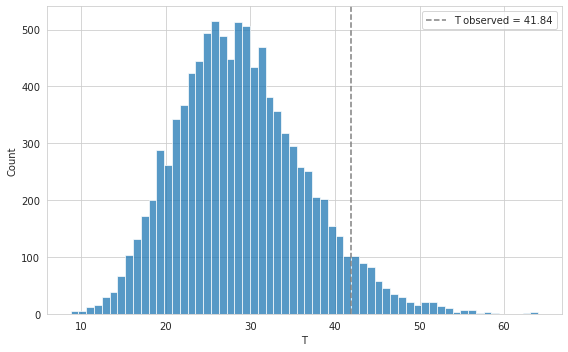
\includegraphics[width=0.6\textwidth]{hw5-2.png}
  \captionsetup{justification=centering}
  \caption{The discrete estimation of the un-normalized log-likelihood function $g(T(x), \theta)$ using the sufficient statistics. We only plotted the points in that we have at least 15\% of the maximum log-likelihood score to highlight the region.}
  \label{fig:sufficient-logl}
\end{figure*}

\paragraph{(c)}

\end{document}